% This file was converted to LaTeX by Writer2LaTeX ver. 1.4
% see http://writer2latex.sourceforge.net for more info
\documentclass[a4paper, 12pt]{article}
\usepackage[utf8]{inputenc}

\usepackage[T1]{fontenc}
\usepackage{times}
%\usepackage[T1]{fontenc}
%\usepackage{lmodern}
\usepackage[english]{babel}
\usepackage{amsmath}
\usepackage{amssymb,amsfonts,textcomp}
\usepackage{array}
\usepackage{hhline}
%\usepackage{setspace}
%	\linespread{1.5}
	%\begin{singlespace} et end singlespace
\usepackage[pdftex]{graphicx}
\usepackage[hidelinks]{hyperref} % to hide ugly links use
\def\UrlBreaks{\do\/\do-} % To break urls at the end of the line
\usepackage{subcaption}
\usepackage{setspace}
% For bibliography:
\usepackage[
%    natbib = true,
%     backend=bibtex, % this OR biber
backend=biber,
isbn=false,
url=false,
doi=false,
eprint=false,
%    style=numeric,
%style=authoryear,
style=authoryear-comp,
sorting=ynt, % sorts names in citations by year, name, then title
sortcites = true, % to avoid first names, but check disambiguation in the very end:
uniquename=false,
uniquelist=false,
maxbibnames=3,    
maxcitenames=2 % to put "et al" after a few authors
]{biblatex}
\renewcommand*{\nameyeardelim}{\space} % to remove the coma in textcite (bug work around)
\bibliography{bibzotero}
% To clear the "note" field:
\AtEveryBibitem{%
	\clearfield{note}%
}
\AtEveryBibitem{%
	\clearlist{language}%
}

\renewbibmacro*{name:andothers}{% Based on name:andothers from biblatex.def
	\ifboolexpr{
		test {\ifnumequal{\value{listcount}}{\value{liststop}}}
		and
		test \ifmorenames
	}
	{\ifnumgreater{\value{liststop}}{1}
		{\finalandcomma}
		{}%
		\andothersdelim\bibstring[\emph]{andothers}}
	{}}
\emergencystretch 2em % To avoide overfull boxes
\renewcommand{\baselinestretch}{1.5}

%\topskip=40pt
%\parskip=10pt
%\parindent=0pt
%\baselineskip=15pt

\usepackage{geometry}
\geometry{a4paper, portrait, left=2.5cm, right=2.5cm}
%%\textwidth=12.978986403cm % golden ratio
%%\addtolength{\oddsidemargin}{1cm}
%%\addtolength{\evensidemargin}{1cm}
%%%\addtolength{\textwidth}{-2cm}
\addtolength{\topmargin}{-0.5cm}
\addtolength{\textheight}{1.5cm}

\begin{document}
\title{Mate-copying in Drosophila:\\ a matter of taste or disgust?}		
\begin{figure}
	\vspace{-1cm}
	\hspace{-2cm}
	
\includegraphics[width=20cm]{images/triche}
	
\end{figure}

\vspace*{3cm}


\begin{center}\huge Mate-copying in Drosophila:\\a matter of taste or disgust?\end{center}


\vspace*{1cm}

\begin{center}Guillaume Lespagnol\end{center}


\begin{center}Master 2 - Ecologie Evolution 2018-2019\end{center}

\vspace*{2cm}

Stage de recherche effectué dans le laboratoire Evolution et Diversité Biologique (EDB), Université Toulouse III-Paul Sabatier, sous la direction de \underline{Guillaume Isabel et Magdalena Monier.}
\vspace*{2cm}

\textit{Soutenu le 7 juin 2019 devant la
commission d'examen. Le présent rapport constitue un exercice 
pédagogique qui n'engage en aucun cas la responsabilité du laboratoire 
d'accueil.}





   
     \setcounter{page}{1} %Start the actually document on page 1
	
	
	\clearpage
	
	
 \begin{LARGE}
 	Acknowledgements
 \end{LARGE}
 
 \bigskip
	First, I would like to thank Magdalena Monier for her patience and kindness. She helped me a lot for all the duration of the internship. As much on the practical level, during the experiments, as theoretical for the analysis of the data, the writing of the report and the comprehension of the subject.
	
	Secondly, my thanks go to Guillaume Isabel, who, even though he was more distant, was very kind and patient to me and my lack of knowledge about neuroscience. He was a great help in understanding the neuroscience part of this internship and I had fascinating discussions with him.
	
	I would like to thank Sabine Noebel and Arnaud Pocheville. Sabine for her help and valuable advice that allowed me to be more rigorous and efficient in data collection. Arnaud Pocheville for bringing me very pertinent thoughts and introduced me to the dark arcana of GIT and LateX.
	
	Finally, Etienne Danchin, for his adices and without whom this internship would not have been possible.
	\clearpage
 \begin{LARGE}
Fiche déclarative
 \end{LARGE}


	Je déclare sur l'honneur l’exactitude des faits énoncés ci-dessous:
	
	Le projet et les hypothèses ont été préalablement conçus par mon équipe d’accueil avant mon arrivée et je n’ai pas pris part à leurs élaborations.
	
	Concernant la collecte de données, j’ai récolté 1149 lignes de données pour 1750 au total. Magdalena Monier, Laura Fargeot et Sabine Noebel ont collecté le reste des données. Pour la deuxième expérimentation, j’ai modifié le dispositif classique afin de pouvoir chauffer les mouches à la température désirée. 
	Pendant la période de récolte des données (début janvier- début mai) j’ai effectué l’élevage des mouches de la lignée CANTON-S, ainsi que des lignées mutantes requises pour mon expérience pendant le mois d’avril. J’ai dû pour cela, avec l’aide de Magdalena Monier, anesthésier et trier les mouches mutantes afin de ne conserver que les phénotypes d’intérêt. J’ai aussi participé à la fabrication des milieux d’élevage des mouches, avec l’aide de Nathalie Parthuisot, Magdalena Monier et Sabine Noebel.  
	
	La méthode d’analyse des données m’a été communiquée par Magdalena Monier, qui m’a également fourni une partie du script utilisé pour l’analyse. J’ai rentré les données sur Excel (excepté celle de Laura Fargeot) et je les ai analysées grâce au logiciel R. Magdalena Monier a également vérifié la cohérence des analyses de la première expérience.
	
	Enfin, j’ai rédigé l’ensemble du présent rapport. Magdalena Monier a corrigé les parties Résumé, Introduction, Matériel et Méthodes et Résultats sur la forme et le fond. Guillaume Isabel a corrigé après relecture par Magdalena Monier les parties Introduction et Matériel et Méthodes sur le fond. La discussion n’a été corrigée par personne d’autre que moi. 

\clearpage
	
	
	\vspace*{2cm}
	\tableofcontents
	
	\clearpage

\section{Abstract}
\begin{singlespace}
In many species, the preference for sexual partners is influenced by the choice of 
conspecifics, this process is called mate-copying. It allows individuals to indirectly learn information about the quality of a potential mate, by observing its success with conspecifics. Mate-copying has been shown in \textit{Drosophila melanogaster}, which allows the detailed study of its mechanisms. If neuronal mechanisms of direct (non-social) learning are well known in this species, social learning is still widely misunderstood. Mate-copying, with its simple protocol developed in the lab, gives us a chance of unravelling the mechanisms of a social learning. We first investigated the type of information involved in mate-copying: positive information, copulation of the demonstrator or negative information, rejection by the demonstrator. We divided these two components of mate-choice to see if separately they allowed mate-copying. We then sought to know which neural pathway was involved in mate-copying. Using UAS/GAL4 technology, we silenced two neuronal groups involved in the formation of direct associative memory, TH and Ddc neurons. We found that showing the acceptance of a partner, but not the rejection, can elicit mate-copying. Moreover, TH neurons are required for mate-copying while Ddc are not. This last result is surprising, as TH is involved in aversive memory during direct learning, whereas we have shown that it is a positive information that drives mate-copying. Therefore, social and non-social learning may not share the same neural mechanisms. Such results raise many questions about the evolution of social learning, and the mechanisms that enabled it.
\end{singlespace}
\medskip
\begin{large}
\textbf{Résumé}
\end{large}

\begin{singlespace}
\noindent{Dans de nombreuses espèces, la préférence envers les partenaires sexuel est influencé par le choix des conspécifiques, ce processus est appelé mate-copying. Cela permet aux individus d'apprendre indirectement la qualité de leurs partenaires potentiels en observant leurs succès avec ses conspécifiques. Le mate-copying a été montré chez \textit{Drosophila melanogaster}, ce qui permet l'étude détaillée de ses mécanismes. Si les mécanismes neuronaux d'apprentissage direct (non-social) sont bien connus chez cette espèce, c'est loin d'être le cas pour l'apprentissage indirect(social). Le mate-copying, par la simplicité de son protocole expérimentale, nous donne une chance de mieux comprendre les mécanisme de l'apprentissage social. Nous nous sommes d'abord intéressés au type d'informations échangés dans le mate-copying: positive, la copulation de la démonstratrice ou négative, le rejet par la démonstratrice. Nous avons divisé ces deux composantes du choix du partenaire pour voir si elles permettaient séparément le mate-copying. Nous avons ensuite cherché à savoir quels groupes neuronaux étaient impliqué dans le mate-copying. En utilsant la technologie UAS/GAL4, nous avons bloqué l'expression de 2 groupes de neurones impliqués dans la mémoire associative direct, TH et Ddc. Nos résultats montrent que c'est la copulation et non le rejet d'un partenaire qui permet le mate-copying. De plus, le groupe de neurones TH est requis pour la copie de partenaire, mais pas Ddc. Ce résultat est surprenant car TH est impliqué dans la mémoire aversive de l'apprentissage direct, alors que nous avons montré que c’est une information positive  qui permet le mate-copying. Par conséquent, l'apprentissage social et non social ne partagent pas les mêmes mécanismes neuronaux. De tels résultats soulèvent de nombreuses questions sur l'évolution de l'apprentissage social et sur les mécanismes qui l'ont permis.}
\end{singlespace}	
\section{Introduction}


There are few things as extravagant as the traits develloped by sexual selection. In somes species, the access to the reproduction is obtained
 by harm and it is a matter of weight, strength or weapons \parencite{anderson_grey_1985, clutton-brock_functions_1982}. While in others it is by charms and the opposite sex chooses the breeders, in a much more peaceful contest.  Mate-choice (i.e intersexual selection) can lead to captivating and highly complex traits to attract the opposite sex, such as courtships or songs in birds \parencite{danchin_ecologie_2005}. Nevertheless, many species do not exhibit such traits and the choice is based on much more discreet signs. Yet, as stated a century ago by A.R Fisher: “The most difficult and important act of choice is the choice of a mate” \parencite{fisher_evolution_1915}, any mistake can be very expensive since it directly impacts individual’s offspring. To avoid mistakes, many species have acquired the capacity to learn from the observation of others and can therefore use social learning in numerous decision-making processes.

Social learning can take many forms as the transmission of information can be
intentional (teaching), or not. The latter is simpler since it does not require an active and intentional participation of the demonstrator. Copying is likely to be more common, and even exists in non-social invertebrates\parencite{coolen_social_2005, mark_how_2010}. Many behaviors can be copied, whether trivial \parencite{van_leeuwen_group-specific_2014} or decisive for the individual’s fitness \parencite{mery_public_2009}. It’s particularly beneficial when individual learning is costly (time consuming or dangerous; see also\parencite{webster_social_2008}) as in mate-choice. Therefore, copying the mate-choice of potentially more experienced conspecifics can be a good solution for naive individuals to avoid the extra costs of individual learning


Mate-copying is a form of social learning in which the observation of a sexual interaction in conspecifics biases the subsequent mate-choice decision of the observer \parencite{brown_fish_2011}. It has been first demonstrated in fishes \parencite{dugatkin_reversal_1992}, followed by observations in many vertebrates \parencite{galef_mate-choice_1998, yorzinski_same-sex_2010} and recently in invertebrates \parencite{mery_public_2009, fowler-finn_complexities_2015}. Its benefits are double-sided as it facilitates the decision of the mate-choice of naïve individuals and make sure that their descendants will be preferred by conspecifics. By reproducing with a partner of the most preferred phenotype, their descendants will have chances to possess in their turn the preferred trait.
Interestingly, in population with genetic preferences, mate-copying can override them \parencite{dugatkin_interface_1996, witte_male_1998}. At a larger scale, mate-copying can even shape preferences of entire populations: a trait-based preference, transmitted vertically and horizontally and possibly for a long time can lead to long-lasting local tradition that can be considered as a form of animal culture\parencite{brooks_importance_1998, danchin_cultural_2018}.

The existence of culture in non-human species has long been disputed \parencite{laland_animals_2003} but is increasingly accepted among scientists \parencite{aplin_experimentally_2015, whitehead_geneculture_2017}. The list of animals for which a form of culture was documented is growing constantly \parencite{van_schaik_orangutan_2003, thornton_multi_2010, whiten_culture_2017} , and one of the most recent may surprise many, \textit{Drosophila melanogaster} \parencite{danchin_cultural_2018}.  Very few, if none, species have been studied as deeply, with as extensive knowledge in every scientific field (genetics, development, neuroscience…) as \textit{Drosophila melanogaster}. This species of flies has been used for more than a century as a model organism in many different fields of biological sciences.  Its brain structure has been widely studied and is very well understood, making this species a great model to study neuronal mechanisms of complex behaviour. Thus, existence of mate-copying in this species represents a wonderful opportunity to understand the obscure neuronal roots of an evolutionary process widely shared among animals.  

There are only two ways to learn, direct learning (the individual learns by himself) or indirect learning (the individual learns from others). Since a century, the works of Pavlov and Skinner have led to considerable advances in the study of associative learning mechanisms \parencite{pavlov_conditioned_1927, skinner_behavior_1938}. Associative learning can be studied using two main methods: pavlovian conditioning and operant conditioning. In pavlovian conditioning experiments, it is possible to teach the animal to react to a previously neutral stimulus, by associating for example a sound (neutral cue) with the presence of sugar (appetitive cue). In operant conditioning, it is possible to teach them to change their behavior in response to a stimulus. For example, by exposing them to an electric shock as they move in a specific direction. Contrary to Pavlovian, operant conditioning requires a specific action of the animal which is active. With the help of genetic and neuronal tools, it is possible to know the neuronal groups involved in these behavioral associations. In drosophila, depending on the valence of the stimulus (either appetitive or aversive), different groups of neurons are involved in the learning process \parencite{vogt_shared_2014, busto_olfactory_2010}. But only few studies focused on indirect learning and its mechanisms.Therefore, our first step was to test whether mate-copying implies aversive or appetitive memory. During a classic mate-copying experiment, the demonstration contains several types of information, the acceptance of one male and the rejection of another. We considered that a rejection represents a negative stimulus and acceptance of copulation a positive stimulus for an observer female. So, we created two treatments by presenting to an observer, a male rejected by a female ("Rejection" treatment) or a male accepted by a female ("Acceptance" treatment), and we measured the observer’s inclination to copy. 
	
In a second part, we went deeper into the neuronal mechanisms of mate-copying by searching which group of dopaminergic neurons is required for mate-copying. The neuronal mechanisms underlying non-social visual and olfactory learning are very well known in drosophila (reviewed in \textcite{guo_vision_2017} and \textcite{cognigni_right_2018}). Regarding their roles in non-social learning, two brain structures are particularly prone to be involved in mate-copying, the central complex and the mushroom bodies. The central complex localized in the center of the insect brain plays a major role in decoding visual information. It receives visual inputs from the rest of the brain and controls vision-related behaviors, memory and learning. The mushroom bodies are formed by two symmetrical groups of approximately 2500 neurons in the center of the insect brain. Several studies about its structure showed that it can be divided in different sub-areas: calyx, pedunculus, medial lobes and vertical lobes \parencite{aso_neuronal_2014}(voir figure~\ref{fig:brain}). Mushroom bodies are an integrative center involved in learning, memory and decision-making. It has been compared to the hippocampus of mammals due to the similar role they play in learning \parencite{strausfeld_evolution_1998}.
Notably, a recent study found that \(\gamma\) lobes are required for visual associative memory \parencite{ vogt_shared_2014} which is consistent with previous studies showing that neurons involved in appetitive and aversive memories are heavily connected to \(\gamma\) lobes \parencite{claridge_writing_2009, burke_layered_2012}. 

	\begin{figure}
	\centering
	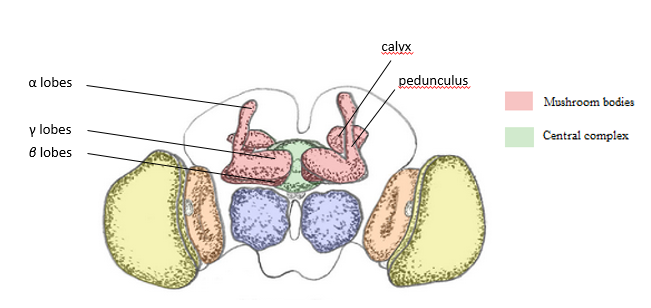
\includegraphics[width=0.9\textwidth]{images/brain}
	\caption{Schematic representation of \textit{Drosophila melanogaster} brain.\\
		Adapted from Koniszewski \textit{et al.,} 2016
		}
	\label{fig:brain}
\end{figure}

On the contrary, despite a rich repertoire of well-studied social processes \parencite{pasquaretta_how_2016, teseo_fighting_2016, dawson_social_2018}, neuronal mechanisms of social learning are still poorly understood.  However, a recent study found that dopamine is required in mate-copying \parencite{monier_dopamine_2018}. Dopamine is a neurotransmitter produced and released by different clusters of dopaminergic neurons in the fly brain, and drives a variety of brain functions among which the formation of appetitive and aversive memories \parencite{riemensperger_punishment_2005, sitaraman_serotonin_2008, alekseyenko_targeted_2010, berry_dopamine_2012, yamamoto_dopamine_2014}. We do not know which dopaminergic neurons are involved in mate-copying, but a reliable method has been developed, allowing to study specifically the role of a group of neurons, UAS/GAL4 technology. UAS/GAL4 is a genetic tool developed in \textit{Drosophila melanogaster}, that allows to mark specific neurons (voir figure~\ref{fig:mcnb}). UAS is an enhancer sequence that activates the transcription of the downstream gene when the transcription factor GAL4 binds it. GAL4 is a transcription factor that can be expressed in a specific type of cells, by placing its sequence after specific enzyme promoters. A huge diversity of GAL4 drivers have been developed to target any cell type in the fly body at any developmental stage.In this study we used two of them: TH (tyrosine hydroxylase) and Ddc (dopa-decarboxylase). Both are enzymes involved in the synthesis of dopamine, their drivers thus mark dopaminergic neurons. But the GAL4 tool is not perfect, and all the dopaminergic neurons are not labeled by TH and Ddc, and \textcite{liu_subset_2012} showed that they do not overlap. TH is mainly expressed in the neuronal cluster PPL1 and Ddc in the PAM cluster. They have been shown being involved in visual direct associative learning \parencite{vogt_shared_2014}; TH for aversive memory and Ddc for appetitive memory. In 2015 \textcite{avargues_information_2015} hypothesized that social learning, and therefore mate-copying, could be assimilated to a simple associative learning, with copulation acting as the unconditional stimulus and male color as the conditional stimulus. The results of \textcite{monier_dopamine_2018} tend in this direction, by showing that dopamine is likewise involved in mate-copying. It is therefore plausible that, as for direct learning, TH and Ddc neurons are also involved in mate-copying. Thus, the aim of our second experiment was to test if the neurons labeled by Ddc and TH are involved in mate-copying.
	
		\begin{figure}
		\centering
		\includegraphics[width=0.7\textwidth]{images/guas}
		\caption{Schematic representation of the GAL4/UAS system.\\ 
			GAL4 transgene is inserted in downstream of a molecule-specific promoter, here Tyrosine-Hydroxylate (TH) or DopaDecarboxylase (ddc). GAL4 is thus expressed in the same tissues as these molecules. Thus GAL4 transcription factor will activate the enhancer UAS (Upstream Activating System) which is followed by the gene of interest, here shibire, and will allow the expression of the corresponding molecule in response to GAL4. This molecule will be expressed only in tissues where GAL4 is present.}
		\label{fig:GUAS}
	\end{figure}
		
Thanks to \textcite{kitamoto_conditional_2001}, we know that UAS-GAL4 technology with the thermosensitive Shibire protein can be used to block specific sets of neurons (see also \textcite{kosaka_reversible_1983, kasuya_neuronal_2009}). Precisely, Shibirets is a thermosensitive variant of Dynamine that blocks synaptic transmission at restrictive temperatures (over 30°C) in a reversible manner \parencite{kosaka_reversible_1983}. Thus, when mutant flies containing both transgenes UAS-shits and GAL4 are exposed to a restrictive temperature (33°C), neurons where GAL4 is expressed are silenced. Our goal was to use this technique to study mate-copying. We used mutant flies with the transgene UAS-shits, and TH-GAL4 or Ddc-GAL4 (allowing expression of the GAL4 transcription factor specifically in TH neurons or Ddc neurons respectively). This allowed us to have a temporal control on TH and Ddc-labelled neurons activity and to silence them during the demonstration in order to see if they are required in mate-copying (for more details, see "Fly strains and crossings" section). We thus created two treatments, depending on the group of neurons silenced, and measured mate-copying scores in each of them. If one group is involved in mate-copying, the corresponding treatment will not display mate-copying (score similar to random choice), due to the incapacity of mutants to learn.



	
	

	

	\section{Material and Methods}
	
	\bigskip

	\subsection{Fly maintenance}
	
	We used the common Canton-S strain of \textit{D.melanogaster} (wild-type, and UAS / GAL4 lines described above). Flies were raised and kept in 30 ml tubes containing standard corn flour-yeast-agar medium at 25° ± 1°C and 56 ± 4 \% humidity with a 12:12H light:dark cycle. Humidity and temperature were controlled and adjusted continuously with two independents automatic humidifiers and one manual heater. Medium was cooked every 3 weeks and stored at 4°C until use. Flies were manipulated with a hand-made mouth aspirator made of a glass pipette, tubing and gauze.
	
	Every morning, adult flies were removed from the breeding vials so that the newly emerged flies collected within the 6-8 hours were virgin. For Canton-S strain, 120 males and 120 females were used daily for breeding (20 tubes with 6 males and 6 females in each) and all other adults were euthanized in a freezer. For mutant strains, all adults were used for breeding. 
	
	Virgins were sexed without anesthesia, by gentle aspiration and then kept in unisex groups of 7 females or 14 males until experiments. Both demonstrator and observer flies were 3 or 4 days old. Males and females were used only once as females are reluctant to re-mate \parencite{chapman_sex_2003} and reject males they just saw copulating \parencite{loyau_when_2012}. After experiments, all flies were put in a food vial and cold-euthanized at the end of the day.
	
	\subsection{Fly strains and crossings}
	

	
	Mutant lines (described above) for the second experiment were obtained by crossing homozygous lines.
	UAS-Shits is a transgene that contains an GAL4-specific enhancer,UAS (Upstream Activating Sequence) driving the production of Shibire protein in cells where GAL4 is present. Shibire is a thermosensitive protein that inhibit neuronal activity at restrictive temperature (30°C) by preventing vesicle recycling \parencite{kitamoto_conditional_2001}. Ddc-GAL4 and TH-GAL4 drive production of a transcriptional activator (GAL4) only in specific subsets of dopaminergic neurons. GAL4 activates the expression of genes downstream to UAS. Ddc-GAL4 labels neurons involved in appetitive olfactory memory:the blockade of these neurons by Shibire protein has been shown to impair the acquisition of such memory at restrictive temperature\parencite{kosaka_reversible_1983}.TH-GAL4 labels neurons involved in aversive olfactory memory \parencite{liu_subset_2012}.
	
	As \textit{white} recessive mutation w\textsuperscript{-} impairs fly vision \parencite{gotz_optomotorische_1964}, we used mutant females with one wild-type copy of the white gene for the experiments. To do so, we crossed w\textsuperscript{+};;Shi\textsuperscript{ts} males with females from each Gal4 line. To obtain w\textsuperscript{+};;Shi\textsuperscript{ts} strain from a w\textsuperscript{-};;Shi\textsuperscript{ts} strain, we crossed males w\textsuperscript{-};;Shi\textsuperscript{ts} with females w\textsuperscript{+};;TM2/TM6b over two generations and with CO\textsubscript{2} anesthesia, and we isolated homozygous w\textsuperscript{+};;Shi\textsuperscript{ts} progeny.
	
	Thus, we used two mutant genotypes, Ddc-GAL4/w+;;UAS-Shi\textsuperscript{ts}/+ and w+/w-;;UAS-Shi\textsuperscript{ts}/TH-GAL4 ,obtained by crossing homozygous lines. 
	
	TH-GAL4 and Ddc-GAL4 lines were provided by Guillaume Isabel in the same Canton-S background as the Wild-type strain.


	\subsection{General experimental procedures}
	
		\begin{figure}
		\centering
		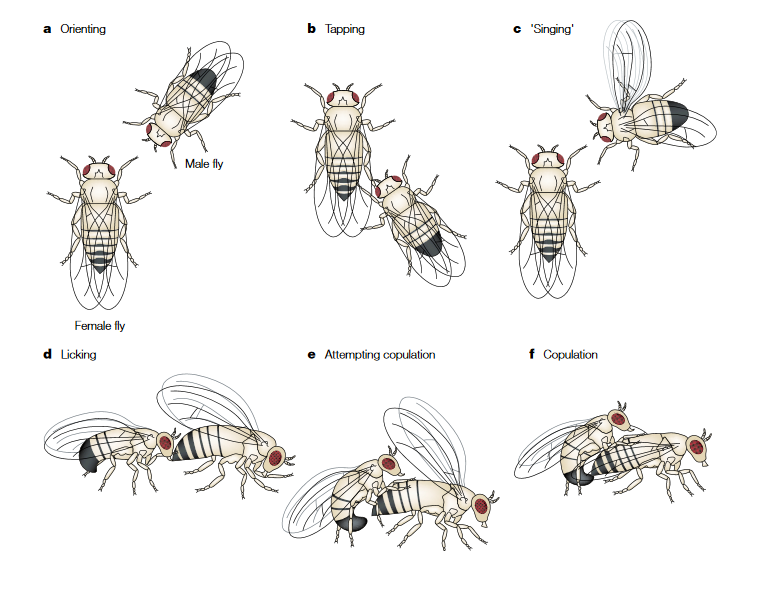
\includegraphics[width=0.7\textwidth]{images/courtcomp}
		\caption{The different phases of courtship behaviors of males \textit{D.melanogaster}.\\
			a: The male fruit fly orientates towards the female and follows her
			b: taps her 
			c: sings a species-specific courtship song by vibrating one wing
			d: finally, he licks the genitalia of the female 
			e: curls his abdomen in an attempt to copulate with her.
			Adapted from Sokolowski 2001.}
		\label{fig:court}
	\end{figure}
	Artificial male phenotypes were created by dusting virgin males with pink or green powder \parencite{mery_public_2009}. Each vial of males was randomly assigned to a color. Before the experiment started, males were placed in a clean vial to remove the excess of dust for at least 20-30 min. Experiments took place in the same tube set-up and a similar but slightly modified speed-learning protocol than described in \textcite{dagaeff_drosophila_2016} (Voir figure~\ref{fig:classic}, see also specific experiment section).
		

	Demonstrator and observer flies were placed in two compartments of double plastic tubes, separated by a thin glass partition and closed by cotton plugs. All replicates were run in blocks of six trials with cardboard barriers between experimental set-ups, to prevent information exchange between the flies and disturbance from the surroundings. 
	
	During the demonstration, we always showed two different male phenotypes (color) to the observer females, with one favorite that copulated with the demonstrator female. If demonstrator females refused to copulate, the trial was discarded. Specifics of demonstrations for each experiment are described above (see specific experiment section).
	
	Once the demonstrations were over, we started the mate-copying test by introducing a couple of colored virgin males (one of each color) in front of the observer female and we removed the partition, allowing the female to freely choose between males for 30 min. The partition was put back in place when all three flies were in the same side of the tubes, to promote proximity between flies. During that time, we recorded the time of first courtship for each male, the time when copulation started and the color of the chosen male. The onset of the courtship was defined as the first wing-extension of a male (Voir Figure~\ref{fig:court}).
	
	

	\begin{figure}
	\centering
	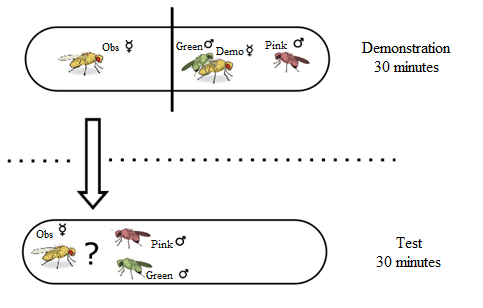
\includegraphics[width=0.6\textwidth]{images/classic}
	\caption{Classic mate-copying protocol.\\ 
		During demonstration, observer female watches the free choice of demonstrator female. After all copulations ended, demonstrators were removed. Observer females are tested immediately after the end of the demonstration.}
	\label{fig:classic}
\end{figure}

	\subsubsection{Acceptance/Rejection experiment}
	
	During this first experiment, we tested whether mate-copying is achieved through aversive or appetitive memory. To do so, we split the negative and positive information given by the usual mate-copying demonstration. A classical demonstration, in which a demonstrator female chooses between two males, contains a rejection (negative information) of a male and an acceptance (positive information) of the other one. We thus created three demonstration treatments: (1) a "control" where a demonstrator female freely chooses between two males, (2) an Acceptance treatment with one accepted male copulating with a demonstrator female, and (3) a Rejection treatment with one male actively rejected by a female (Voir Figure~\ref{fig:ar}).
	
		\begin{figure}[h]
		\centering
		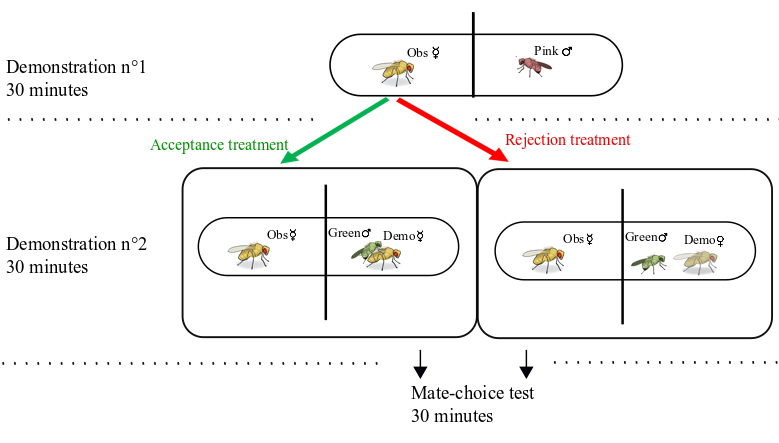
\includegraphics[width=0.9\textwidth]{images/ar}
		\caption{A/R experiment. 
		For acceptance treatment, both demonstrators were virgin, while for rejection treatment, only males were virgin. For control treatment, the observer female is placed in front of an empty tube for demonstration n°1 and face a free choice of the demonstrator female between two males for demonstration n°2. If the female rejected the male during acceptance treatment, it was switched to rejection and if female accepted the male during rejection treatment, it was switched to acceptance treatment. The demonstration order was reversed each day.For each phase, after all copulations ended or 30 minutes, demonstrators were removed.}
		\label{fig:ar}
	\end{figure}
	
	\subsubsection{Neuronal blockade experiment}
	
	This second experiment aimed at exploring the mechanisms underlying the results of the Acceptance/Rejection experiment by discovering one group of dopaminergic neurons involved in mate-copying.
	
	The demonstration was similar to classical protocol (Figure 1), but we used Ddc-GAL4/w\textsuperscript{+};;UAS-Shi\textsuperscript{ts}/+ (treatment “Ddc”) and w\textsuperscript{+}/w\textsuperscript{-};;UAS-Shi\textsuperscript{ts}/TH-GAL4 mutants (treatment “GAL4”) as observer females. We thus had a temporal control on specific sets of neurons presumably involved in appetitive (Ddc) or aversive (TH) memory. During the demonstration and 30 minutes before, observer mutant females were heated to a restrictive temperature of 33°C, thanks to a heating mat under the tube of these females. At 33°C, Shibire protein blocks the neurons in which it is expressed, and thus the acquisition of appetitive memory should be blocked in observer females of “Ddc” treatment, and the acquisition of aversive memory in “TH” females. 
	
	After all copulations ended, demonstrator males and females were removed. Observer females were then stored individually in clean tubes at 25°C for 3-4 hours to ensure that labelled neurons are no more blocked, then we proceeded to a classical test at 25°C.


	\subsection{Mate-copying score}

	As in previous studies \parencite{dagaeff_drosophila_2016, nobel_mate-copying_2018,monier_dopamine_2018}, a mate-copying score evaluated female’s tendency to copy the choice of the demonstrator. A mate-copying score of 1 was assigned to females that copulated with the color preferred by demonstrator females and a score of 0 in the opposite case. For each treatment, a mate-copying index was calculated as the mean of mate-copying scores per treatment, a random choice indicated by a value of 0.5. As in previous studies \parencite{dagaeff_drosophila_2016, nobel_mate-copying_2018,monier_dopamine_2018}, all replicates where only one male courted the female before copulation were discarded because in these situations the female was not unambiguously in a position to make a choice between the two colors.

	\subsection{Statistical analyses}

	All statistical analyses were performed with the R software version 3.5.1 (R Core Team, 2018).
	For each treatment, the difference from a random choice was tested with a binomial test. Mate-copying scores were then analyzed in a generalized linear mixed model (GLMM, package lme4 \parencite{bates_fitting_2015}). Starting models contained the following fixed effects: treatment, normalized air pressure (air pressure in Toulouse-Blagnac weather station, at the time of the beginning of the experiment, minus mean air pressure), normalized air pressure variation within the six preceding hours and all interaction between these three variables, experimenter effect and its interaction with treatment. A random “block” effect was also introduced in the models to account for the non-independence of observer flies from the same block of 6 tubes-set up trained and tested in parallel. The significance of fixed effects was tested using Wald chi-square tests included in ANOVA function (car package, \textcite{fox_r_2018} ). Model simplification was achieved by successive withdrawal of the non-significant terms in a backward selection approach, using P-values and starting with the highest-order interaction. The final model was chosen as the one with the lowest Akaike Information Criteria (AIC, Akaike, 1969). Comparisons between treatments were done using post-hoc X² tests. 
	
	\subsection{Verification of labeled neurons in Ddc-GAL4 mutants}
	
	In view of the results of the neuronal blockade experiment, we wanted to check GAL4 expression pattern in Ddc-GAL4 flies. No verification has been conducted so far for this strain in our Canton-S background, contrarily to TH-GAL4 strain ( Isabel,G Personal Communication). We created Ddc-Gal4/+;;UAS-GFPmCD8 /+ flies, expressing the green fluorescent protein (GFP) in cells expressing Gal4. We then collected adult females and dissected the whole brain in PBS (phosphate buffered saline), then mounted it in PBS for confocal acquisition with a (Leica TCS SP5), at 40x, under green light (488nm), with a z-interval of 1.01 µm. Z-projection of the picture was done using ImageJ (Version 1.52o).
	
	
	\subsection{Ethical statements}

	Behavioral observations of \textit{D. melanogaster} required no ethical approval and complied with French laws regarding animal welfare. We kept the number of flies used in this study as small as possible. We handled flies by gentle aspiration without anesthesia to minimize damage and discomfort. After the experiments, individuals were euthanized in a freezer at -20°C.

	\section{Results}

	\subsection{A/R Experiment}
	\label{subsec:AR-experiment}

	For this experiment, we tested 850 females among which 530 copulated during test, including 192 with double-courtship, 64 for each treatment. First we tested for female's color preference with binomial test but neither in the demonstration (N = 850, 426 females copulated with green males and 424 copulated with pink males; binomial test: P = 0.973) nor the test (N = 530, 270 copulated with green and 260 with pink males; binomial test: P = 0.696) was there any significant difference between the two colors.

	For each treatment, the difference from random choice was tested with a binomial test, Acceptance (where the observer female sees a copulation, N = 64, P {\textless} 0.001) and ``control'' (N = 64, P = 0.03) were both significantly different from random, but Rejection treatment (where the observer female sees a male rejected without copulation, N = 64, P = 0.382) was not (Figure 4).

	To test for the significance of mate copying among treatments, we built a global model including the effects of experimenter, treatment, normalized air pressure (actual air pressure minus global mean of air pressure), normalized air pressure variation (for the last six hours) and the interaction between air pressure and variation of air pressure. The selected model included the effect of treatment, air pressure, variation of air pressure and the interaction between air pressure and its variation. Only the treatment had a significant effect on mate-copying (GLMM, $\chi^2$: $N = 192$, $\chi^2 = 10.447$, $p = 0.005$), air pressure (GLMM, $\chi $²: N = 192, $\chi $² = 0.572, p = 0.449) and variation of air pressure (GLMM $\chi $²: N = 192, $\chi $² = 1.831, p = 0.176) were non-significant. The interaction between air pressure and variation of air pressure was close to be significant (GLMM $\chi $²: N = 192, $\chi $² = 2.946, p = 0.086), as we could have expected in regard of the results of \textcite{dagaeff_drosophila_2016}. No significant difference has been found between ``control'' and Acceptance treatments ($\chi $² = 1.76, P = 0.18; Fig4), but both are different from Rejection treatment (acceptance - rejection: $\chi $² = 11.62, P {\textless} 0.005; control - rejection: $\chi $² = 4.52, P = 0.033; Voir figure~\ref{fig:mcsar}).
	

		\begin{figure}
		\centering
		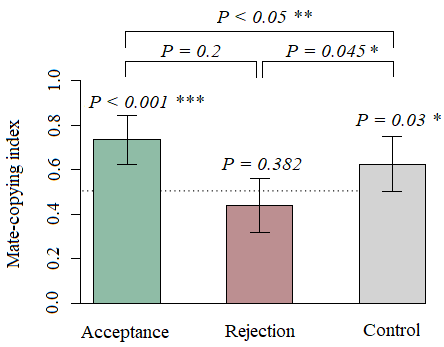
\includegraphics[width=0.6\textwidth]{images/mcsar}
		\caption{Mate-copying index A/R experiment.\\
			 Mate-copying index is calculated as the mean of mate-copying scores for each treatment. Just above the bars: binomial tests of departure from random choice, ***P<0.005, **P<0.01, *P<0.05, NS P>0.05. Two by two comparisons: post-hoc chi-square tests. Test between all groups: GLMM. Dashed lines indicate random choice, numbers inside the bars represent the sample size.}
		\label{fig:mcsar}
	\end{figure}


\subsection{Neuronal blockade experiment}

For this second experiment, we tested 336 females, among which 208 copulated, including 88 with double courtship. Female's color preference was tested with a binomial test, but we found no preference between the two colors in demonstrations (N = 336, 151 females copulated with green males and 185 copulated with pink males; binomial test: p {\textless}0.072) and tests (N = 208, 107 copulated with green and 101 with pink males; binomial test: p {\textless}0.729).

As for the previous experiment, we first tested difference from random choice for each treatment with a binomial test: females from Ddc treatment exhibited a mate-copying score different from random (N = 39, p {\textless} 0.024) while TH did not (N = 49, p {\textless} 0.568)(Fig 5).

To test for the effect of treatment on mate-copying efficiency, we built a global model, including the effects of experimenter, treatment, normalized air pressure (actual air pressure minus global mean of air pressure), normalized air pressure variation (for the last six hours) and the interaction between air pressure and variation of air pressure. The selected model included the effect of treatment, air pressure, variation of air pressure and the interaction between air pressure and its variation.Again, only the treatment had a significant effect on mate-copying (GLMM, $\chi^2$: $N = 88$, $\chi^2 = 4.245$, $p = 0.0394$), while effect of air pressure, variation of air pressure and interaction between air pressure and air pressure (Voir figure~\ref{fig:mcnb}).

Figure~\ref{fig:mcnb} shows a similar cluster marking to those of \textcite{liu_subset_2012}. This allows us to make sure that it is the Ddc neurons that are marked in our mutants. And so that Ddc really does not seem to be involved in mate-copying.

\begin{figure}
	\centering
	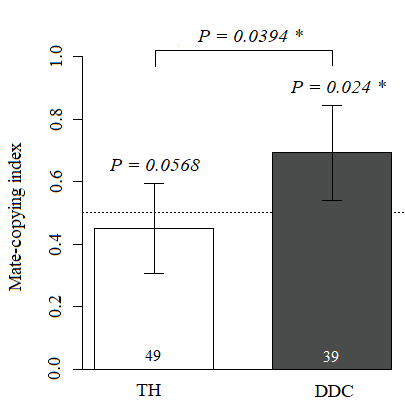
\includegraphics[width=0.4\textwidth]{images/mcnb}
	\caption{Mate-copying index of neuronal blockade experiment. \\
		Mate-copying index is calculated as the mean of mate-copying scores for each treatment. Just above the bars: binomial tests of departure from random choice, ***P<0.005, **P<0.01, *P<0.05, NS P>0.05. Test between the groups: GLMM. Dashed lines indicate random choice, numbers inside the bars represent the sample size.}
	\label{fig:mcnb}
\end{figure}

\begin{figure}
	\centering
	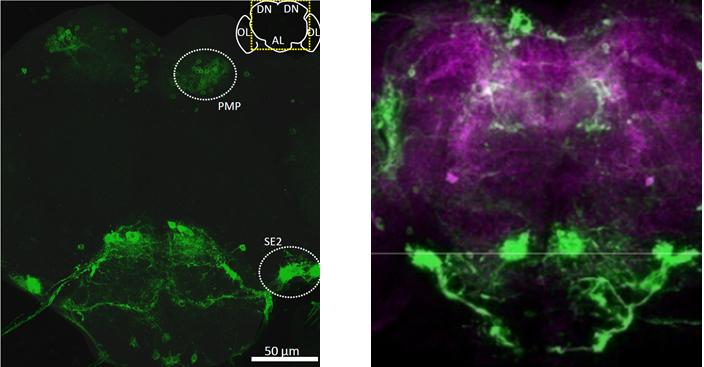
\includegraphics[width=0.6\textwidth]{images/micro}
	\caption{Projection view of the central brain. \\
		On the right: Picture from Liu., \textit{et al} 2012 of Ddc-labbeled neurons)\\
		On the left: Our picture of Ddc-labbeled neurons\\
		OL: optic lobes,
		AL: antennal lobes,
		DN: dorsal neuropils,
		SE2: one cluster of the suboesophagal ganglion,
		PMP: posterior medial protocerebron.\\
	\textit{See}: Figure 5 in supplementary info of Liu, C., Plaçais, P. Y., Yamagata, N., Pfeiffer, B. D., Aso, Y., Friedrich, A. B., ... and Tanimoto, H. (2012). A subset of dopamine neurons signals reward for odour memory in Drosophila. Nature, 488(7412), 512.}
	\label{fig:micro}
\end{figure}

	


\section{Discussion}

So far, mate-copying studies in \textit{Drosophila melanogaster} were based on the acceptance or rejection of different phenotypes by a demonstrator.
Here we showed that the acceptance of a single male is sufficient to induce mate-copying in females drosophila, while rejection is not.
When a female witnessed the acceptance of a male followed by a copulation, she exhibited mate-copying.
In the other case, when the observer female witnessed only a rejection of the male, her subsequent choice was similar to random.
This experience presents some limitations that moderate our conclusions. We used non-virgin demonstrator females in rejection experiment and males can smell that the female has recently mated \parencite{jallon_few_1984}. Even though we made sure the male actively courted the female, it has been shown that the level of courtship is reduced when the male faces females that already mates \parencite{cook_attractiveness_1975, tompkins_conditioned_1983}.
So it is possible that the observer female perceives this difference in courtship and so its inclination to copy may be impacted, leading to the absence of mate-copying in Rejection treatment. It could be interesting to investigate the effect of courtship intensity on mate-copying to go further and be sure that it does not impair the capacity of females to copy.

Several studies in fish have demonstrated mate-copying without copulation between demonstrators, but they are hardly comparable to ours.
In theses studies, the choice of observer female was not showed directly by copulation but only by the fact that she spends more time near one male than with the other \parencite{dugatkin_reversal_1992,galef_mate-choice_1998}. Even if \textcite{bischoff_tail_1985} results show that it is a proxy of the subsequent choices of females, it is not an effective choice. So these results are hardly comparable to ours, especially since the protocols and species are very different.
Yet, it is interesting to note that a study on lekking birds (\textit{Terao tetrix}) found that copulation between demonstrators was needed for mate-copying \parencite{hoglund_mate_1995}. If our results seem to be headed in the same direction, in this study mate-copying was not a matter of biased copulation but of biased attraction to preferred males. In our study, both demonstration and test involved copulation and so it leave little doubt about interpretation.

According to our results, only positive information matters for mate-copying, since the mate-copying index of rejection treatment was not different from random.
In both treatments, only a part of the information was available for the female.
Also, since we used virgin (naive) observer females, they never observed sexual interaction before.
And even though the two male phenotypes were presented during this experiment, observer females saw the demonstrator female interact with only one of them.
The observers in acceptance treatments only saw accepted males, while in rejection treatments they only saw rejected ones.
The observer female in Rejection treatment could not really observe which phenotype is chosen by the demonstrator female, but only the fact that she rejected one phenotype among potentially many (at least two in our experiment).
Therefore, the fact that mate-copying relies on acceptance and positive information rather than rejection and negative information is rational in regard of evolution.
Mate-choice is based on many individual-specific characteristics. For example, in other species, mate-choice can be partly based on genetic characteristics, such as MHC dissimilarity \parencite{wedekind_mhc_1995, landry_good_2001}. In flies, among other reasons \parencite{tennant_causes_2014}, a female can also reject a male if she recently mated \parencite{chapman_sex_2003} or if she saw that the male copulated recently \parencite{loyau_when_2012}.
So in these conditions, for a trait-based mate-copying, the reasons for the rejection can be pointless for other females and uninformative about the male quality, which is potentially excellent.
Whereas for acceptance, both individual specificities and quality of the male led to the copulation, making acceptance much more informative.


\medskip



Once we found on what kind of stimulus mate-copying is based, we tried to understand the underlying neuronal mechanisms. In regard of the results of the previous experiment, we expected Ddc-neurons to be required in mate-copying, but we were wrong.
Surprisingly, we found that TH-labeled neurons are required in mate-copying, while Ddc neurons are not. When heated to a restrictive temperature, Ddc-GAL4 females copied the choice of the demonstrator despite the fact that Ddc neurons was silenced. In the same context, females with TH-GAL4 neurons silenced didn't exhibited mate-copying, with a mate-copying score similar to random. Before to go further in conclusion, we have to keep in mind that a control treatment was not conducted to verify if the flies w+/w-;;UAS-Shits/TH-GAL4 had a mate-copying score different from random (by lack of time). It is possible that the presence of transgenes impair the functioning of the brain and prevent learning even when the flies are not heated to restrictive temperature. Potentially, the incapacity to learn of these flies may do not come from the silencing of these neurons but from a more global neural problem due to the use of mutants.
According to our results, TH neurons are then required in formation of both aversive direct memory and appetitive indirect memory.
Thus, direct and indirect learning involves different groups of neurons.
From an adaptive perspective, it is relevant that social and non-social learning involves different group of neurons. As the stimulus and the appropriate responses are basically different between these two ways of learning. Indeed, even if several personal stimuli come from different sensory cues, they still convey information specific to the individual and should be used as such. The potential responses are more likely to be determined by the valence (positive or negative) of the stimuli than by its nature, for example the fact that it is visual or olfactory (smelling and seeing a predator should lead to similar reactions).
Comparable results have been found recently in rats. \textcite{carrillo_emotional_2018} showed that a specific group of neurons (in anterior cingulate cortex) responded to a social aversive stimulus (pain of conspecifics) but not to an aversive non-social stimulus (a fear-conditioned sound). After deactivation of theses neurons, the observer rat showed reduced freezing (distress behavior) when witnessing pain of conspecifics, but the freezing behavior in response to fear-conditioned sound was unchanged. Similarly to our study, these results underline the fact that response to social and non-social stimulus involves different group of neurons. Even if it's comparable to our study, the nature of stimulus and difference in brain structure makes it difficult to draw solid conclusions. 
Mate-copying can be explained in terms of simple associative memory, where the copulation of observer act as unconditional stimulus (US) and the color of the male as conditional stimulus (CS). Given that dopamine is required in mate-copying \parencite{monier_dopamine_2018}, it possibly convey the US, as in direct associative learning. Moreover, \textcite{avargues_information_2015} showed that Rutabaga protein is essential for US/CS association in direct learning. And recently, Nöbel \textit{et al}(unpublished results) found that Rutabaga, and \(\gamma\) lobes, are required for mate-copying and possibly play a similar role than in direct learning. Our results showing that TH dopaminergic neurons are involved in mate-copying are thus potentially very interesting. We know that on 180 neurons marked by TH-GAL4 only very few innervate the \(\gamma\) lobes(three) \parencite{aso_neuronal_2014}. And so, there is one or some neurons among these three neurons that convey the US of mate-copying to \(\gamma\) lobes.  So it is possible, and this should be the next step in our understanding of the mechanisms of social learning to discover which one, or which of these neurons carry mate-copying US. 


\bigskip

In conclusion, we showed that mate-copying in flies comes from the observation of copulation between conspecifics, and that its neuronal pathway is different from those involved in direct associate learning. If several issues temper our conclusions (such as lack of control and the use of mated females), it does not prevent our results from showing that even after one century spent studying it, much remains to be learned from \textit{Drosophila}.
Our results are of particular interest for next studies that focus on mate-copying mechanisms. First they show that neuronal mechanism of social and non-social learning are not similar, and that much remain to be discovered in this field. Second, it allow study of precise neuronal mechanisms of mate-copying, as for example the identification of the exact neurons that convey the US of mate-copying.From a more pragmatic point of view, given the high homology between human and flies, such studies on social learning and cognition can potentially lead to major discoveries of human concern. Especially, it could lead to a better understanding of disease like autism that comes from deficiency of neural structure linked to social cognition.
More generally, our results have a lot of implications in an evolutionary perspective.
Especially on the mechanisms of evolution of social learning, and on the evolution timings of each type of learning. The fact that the mechanisms of social and non-social learning are different shows that they may have appeared at different times in the evolution of life. Also the fact that is possible to study social learning in flies, a non-social insect, will potentially allow the study of the evolution of social learning through the complexification of the brain. Finally, the study of social learning and cognition in Drosophila hold considerable promises for future. Its ease of study and the knowledge amassed above allows relevant studies and rapid discoveries of mechanisms still poorly known. Notably, in this period when Neo-Darwinism is undermined, the discovery of a form of cultural transmission in this species is an incredible opportunity. Indeed, if the genetic aspect of transmission is now very well known, epigenetic or cultural transmission, which have an impact in evolution that has long been underestimated, are still rather unknown. Thus, as a model of study, the \textit{Drosophila melanogaster} makes it possible to fill this gap thanks to the in-depth study of the mechanisms underlying evolutionary high-impact processes such as social learning. Future studies will be able to take a closer look at social learning mechanisms, which is at the root of cultural transmission.

\clearpage

\printbibliography


\newrefcontext[sorting=nyt] % sorts the bibliography by name first, then year, title

 \end{document}
